\newpage
\section{Work distribution and personal conclusions}
\label{appendix:work_distribution}

%Who did what and when? We can all write something like max 10 lines to say "I did this and this and this" and with whom we did it.

In this appendix section we will describe the work carried on by each of the engineers in the team, after describing the tools that have been utilised throughout the semester.

\subsection{Tools and organisation}
In order to optimally work in an interdisciplinary team as the one we had, different tools have been chosen to help us along the development. We used Trello for any general goal and to do's, Slack for the communication within the team and engineers, GitHub for code versioning, Google Drive for sharing files as well as Teamweek and a nice cardboard panel to organise our timeline and see who is currently working on what.

\subsection{Who did what?}

\subsubsection{Chloe}
In this project, I was in charge of the Firmware and Mechanical Engineering and Soft Electronics. While we did not have many mechanical parts, the textile and soft electronics were very challenging and required very close collaboration (and many trips to ECAL) with our industrial designer Marjane. I was also in charge of building the prototype for each milestone, which happened to be a very tedious work with all the sewing of electronics. Finally, Marjane and I worked together to define optimal specifications for the next iteration of the prototype. This includes imagining the best way to implement hard<->soft connectors, the smallest PCB and best manufacturing methods for the soft PCB. I also developed the Firmware and test protocols for our prototype. For the communication part, I worked alongside Yann who helped me setup the right communication and connectivity protocols. 
%I baked a cake and it was delicious. I went very often to ECAL and did many Skype calls with Estelle and Yann tried to explain his black magic to me. I took orders from Luca for the interactions and gave orders to Simone about the PCB shape.

\subsubsection{Simone}
Focusing only on the engineering field of the project, my contribution will be explored here below. First, I took care of investigating the hardware development kit to be used for the firmware fast prototyping stage. Then, Yann and I collaborated to implement the Wi-Fi communication on the ESP32 development kit with the Arduino IDE, to avoid the numerous difficulties we were confronted with Eclipse. Afterwards, most of the semester was focused on realizing the PCB (schematic, selection of components, etc). Some extra tasks have been handled, such as the sound implementation (to test and select one of the various speakers available at the laboratory), the determination of power consumption, the selection of battery or the first design of the mechanical box (with the idea of detachable module sewed on the plush toy). 

\subsubsection{Yann}
As the Computer Science engineer of the team, my major focus has been on the Software development of the project. I have set-up and managed the official repository of the project on GitHub, for which each engineer contributed with their content. In a first phase I have coded the basic components of the server application in order to have a working communication between clients. Afterwards, I have defined a complete protocol of communication between actors in the network by illustrating a set of rules to translate and construct messages for any requires events. In cooperation with the interaction designer I have developed the final Android APP for the parents, by integrating required functions and visual interfaces into a working software. Speaking of collaboration, I have indirectly supported the other engineers of the team during the Firmware development process. Lastly, I have participated, whenever in my scope of knowledge, to multiple brainstorming and doubts-exchanges during the development with insights on the matter. 
    
\subsection{Our goals for China and next semester}
    \subsubsection{Chloe}
My main goal before China is to find appropriate manufacturing technique and materials for the soft sensors. With Marjane, I would also like to implement a smaller blackbox housing which would define a unique PCB shape, fitting perfectly into our plush toy and minimising the intrusion of the eletronics.
\newline Next semester, I would like to have a fully functional firmware for the plush toy, including saving WiFi SmartConfigs to EEPROM, sleep functions and a nice sound system.

\subsubsection{Simone}
Before leaving for China, my goal will be to mount and test the PCB, in order to spot problems related to the electronics. Then, once in China, the goal will be to get at least 2 fully working prototypes, thus involving 2 working sets of PCBs (main and detachable modules). A later iteration in the next semester is envisioned, in order to shrink the PCB size, to fit the electronics in a smaller encapsulation.
    
\subsubsection{Yann}
In the weeks antecedent the take-off to China, the main objective is to complete the Android APP development. In order to obtain a working demo for the last milestone, major focus has been allocated to the interactive session with the plush toy. More development towards user administration, plush toy pairing and general settings will be needed. After having obtained a first prototype in China, next semester main goal will be to enrich the system from a LAN to a WAN by releasing a public server application accessible from anywhere in the world as intended.
 
\subsection{What I learnt}
    \subsubsection{Chloe} 
I learned how to implement a complete firmware for a connected prototype from scratch while using libraries and existing functions and tweaking them to my needs.I adapted to our designer's working methods and requirements to collaborate successively, and learned how to manage my work and team in a large project with many team members and supervisors with each their own tasks and requirements. 
Moreover, I have learnt a lot about prototyping with new materials and components that are not mainstream, and how to adapt DIY design to a larger-scale prototype.

\subsubsection{Simone}
Considering only the hard technical skills acquired with this interdisciplinary project, I discovered for the first time the entire process to achieve a connected device. In fact, the engineers started from fast prototyping a basic solution with a development kit, before creating our own electronic solution with a custom designed PCB. Furthermore, I learned how the communication world behind a Wi-Fi connection works, with its system architecture involving a server. All this valuable knowledge will be useful for my future professional career, as I plan to work on the medical robotic field, that often involves embedded electronic systems.
    
\subsubsection{Yann}
My experience within the CHIC program have enriched me a lot towards the hardware conception of connected devices in general. Along with the Embedded Systems class of the previous semester, I have understood how development of electronic devices undergoes. Specifically, I have been able to understand the pipeline to design and produce a PCB. Moreover, I have learned how to cooperate with different engineering backgrounds, thanks to double way flow of knowledge exchanges within their own domains. 

\begin{sidewaysfigure}
    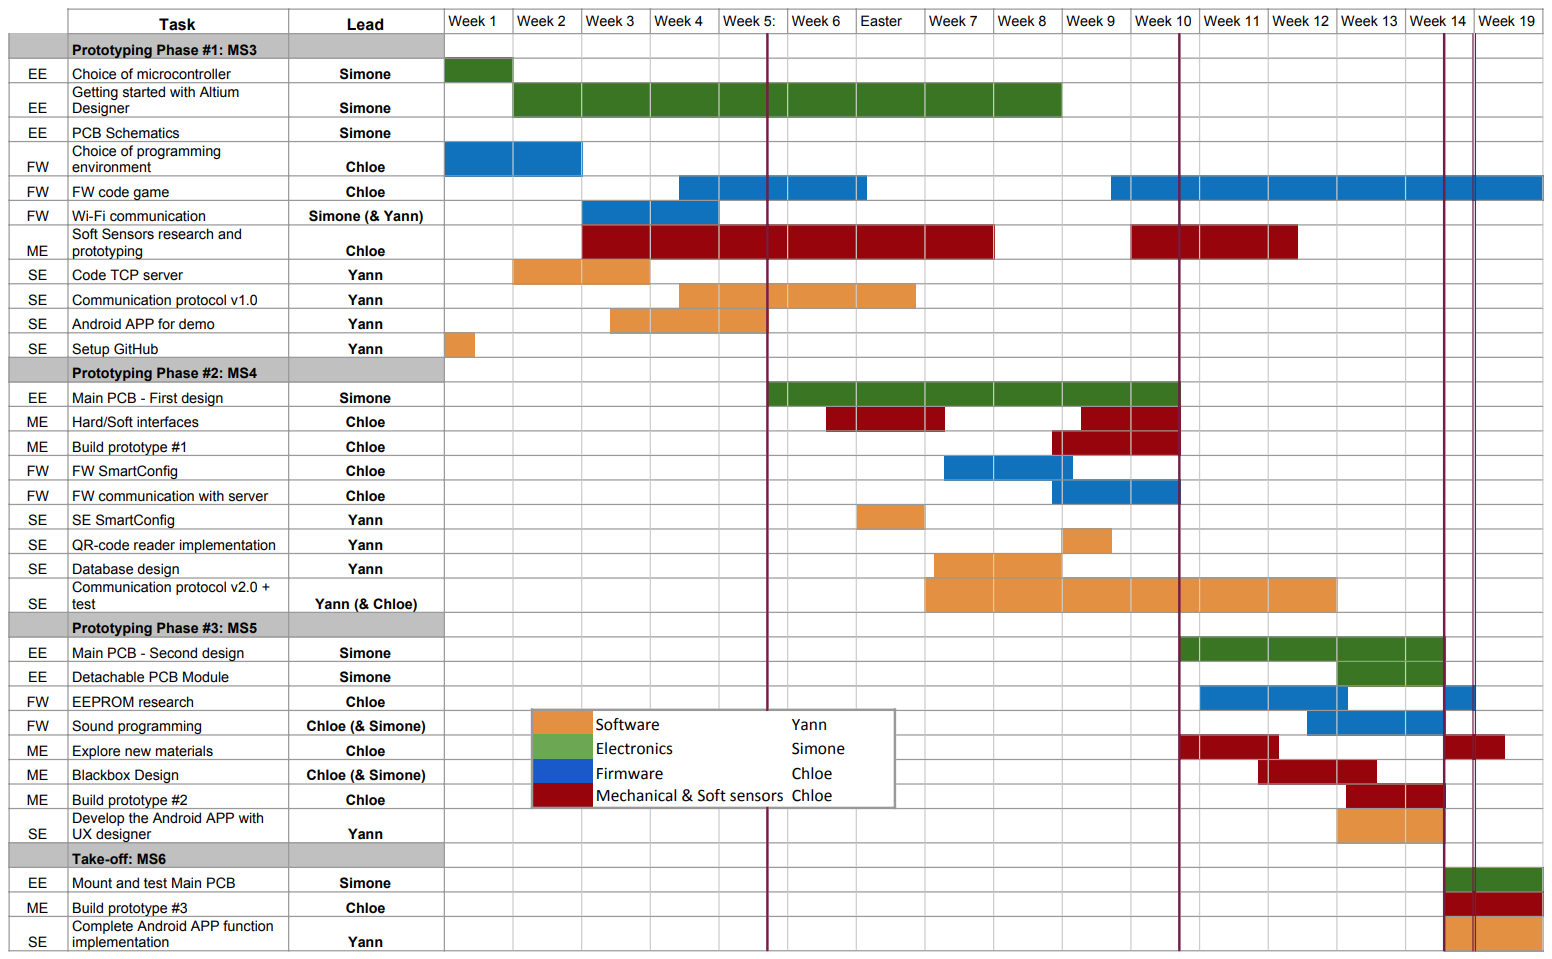
\includegraphics[scale=0.45]{images/gantt.png}
    \caption{Gantt chart for Spring semester}
    \label{fig:gantt}
\end{sidewaysfigure}